\section{Introduction}

% The Introduction includes references to highly-relevant related work,
% i.e., state of the art for the problem you are trying to solve.

% Note: when writing \LaTeX, each paragraph should have a line separated
% between it and the separate paragraph. This causes proper indentation
% and makes the document more readable. Do not end paragraphs with
% \verb/\\/.

%%%%%%%%%%%%%%%%%%%%%%%%%%%%%%%%%%%%%%%%%%%%%%%%%%%%%%%%%%%%%%%%%%%%%%%%%%%%%%%%%%%%%%%%%%%%%%%%%%%%%%%%%%%%%%%%%%%%%%%%%%%%%%%%%%%%%%%%%%%%%%%%%%%%%%%%%%%%%%%%%%%%%%%%

Recent rapid growth of Internet of Things (IoT) technology has made home automation more attractive and more affordable. With smart home devices becoming increasingly more popular, over 20 billion of them are projected to be in use by 2020,~\cite{iot-adoption} numerous smart-home platforms start to appear on the market. Much of the rise in popularity can be attributed to the tremendous utility offered by the smart devices, in which they were able to offer the convenience of automating their home. These devices range from small motion sensors to large digital house appliances such as refrigerator, and enable complex operations across devices (\eg "Turn on the security camera when a motion is detected while I am away from the house"). However, with increasing in convenience of home automation, the associated security risk is also increasing. In addition, automation of smart home opens the attack surface of cyber-physical environment, allowing adversaries to compromise and endanger users' safety without physical access to users' residence. For instance, an adversary can exploit a SSL vulnerability to compromise a door lock, and with that, gaining physical access to a place that is not normally accessible. Just recently, by exploiting the use of common factory default username and password in over 600,000 IoT devices, a historically large scale Distributed Denial of Service (DDoS) attack was launched by Mirai Malware trying to cause a massive Internet shortage.~\cite{tzl+17}

%With increasingly more smart devices coming into consumers' lives, many cloud connected smart devices such as thermostats, security cameras, and smart door locks are being deployed by homeowners. One recent study has predicted that home automation will generate more than \$100 billion in revenue, drawing even more vendors into this ever growing industry.\TONY{Citation here, Tian 2.1}. These new platforms are bringing in more innovating ideas to manages these smart devices. One such example would be Samsung's' SmartThings, which allows smart devices to be connected with a cloud-connected smart hub. Similar vendors typically host third-party IoT apps on their servers, which adds the feature of remote monitoring and controlling to user's home. Most IoT apps can get access to the status of sensors.

%Most Smart home platforms such as Samsung's SmartThings, Google's NEST, and Apple's HomeKit enable home automation through a series of \textit{routines}, trigger-action programs. In essence, these individual trigger-action programs forms the basic building block of complete home automation. Users can specify any \textit{action} events to execute whenever a specific \textit{trigger} condition is satisfied. For example, whenever the user leaves the house (\ie trigger), turn the security camera ON (\ie action).  Previously research has analyzed routines to identify unexpected consequence of home automation and track private data leak. These inspiration often are drawn from the rich domain of Android Security Research. While such an approach may have its advantages (\eg allowing re-use of existing tools and techniques), it has has a critical negative side effect: prior researches generally focus on IoT apps that are build by platform or third-party developers on the public marketplace (\eg SmartApps from the SmartThings marketplace). By focusing only on this specific part of the problem, the prior research fails to account and address the area from the user's side, \ie routines created by end-users.  

End-user programming is often done via a trigger-action framework provided by most Smart Home platforms. These platform vendors often provide an interactive user interface (UIs) that allows user to configure and customize their individual routines. Such design is in a stark contrast to application based platform like Android or iOS, where users depend entirely on applications build by third-party developers. These UIs allow users to create routines by tying together the capabilities of individual devices in the form of trigger-action chains, allowing users who do not have any programming experience to create such programs with ease. However, these user-driven home automations can be problematic since it introduces a set of unexplored scope that may not be apparent from just analyzing IoT apps built by platform vendors or third-party developers. This is illustrated by the dataset we used from a concurrent work which collected from the Computer Science department, in which 107 out of 250, 42.8\%, routines created by 37 users cannot be represented by any of the IoT apps offered by the public SmartThings market. This perfectly demonstrates the existence of a mismatch between user needs and developer-provided functionalities. In addition, this mismatch highlights the unknown nature of user-driven routines and complicates the practical security analysis.

By enabling consumers to control and automate a diverse set of physical objects in their home, home automation platforms are offering a new level of functionality and convenience. While this convenience can be advantageous and beneficial, security flaws in the platform or any smart device can have severe consequences for the safety of users' physical environment. Prior work by Kafle et al.~\cite{kmm+19} has demonstrate the potential for the misuse of routines in Google's NEST platform by being able to perform a lateral privilege escalation attack. During this attack, they were able to first compromise a third-party app that only had access to a low-integrity device (\eg TP Link Kasa Switch), and using the compromised app to trigger an execution of a security sensitive routine, thereby \textit{indirectly} change the state of a high-integrity device (\eg the NEST security camera).This finding motivates the need to assess the security of home automation using a holistic approach.
Similarly, Celik et al.~\cite{cmt18} proposed a static analysis system, Soteria, that can detect side-effects of concurrent execution of IoT apps. Soteria demonstrated that some IoT apps may accidentally trigger an execution of another app, thus leading unexpected and often harmful side-effects. In a similar fashion, IoTMon~\cite{dh18} has demonstrated how malicious applications could deliberately affect environment factors such as the temperature in order to trigger other IoT app. 

Many similar prior works have addressed many IoT security problems by demonstrating the potential benefits to analyze not just IoT apps but also the execution of them. While the lessons and insights from prior work are valuable, they all suffer one common critical limitation: \textit{one-sided perspective}. By analyzing solely on IoT apps from either platform vendors or third-party developers, prior work limited their analysis by relying on a potentially narrow and limited developer's perspective. Although this focus is certainly important, limiting focus to developer's perspective will undoubtedly prevent stakeholders prioritizing more realistic problems that can occur in home automation setup. This limitation motivates the main contribution of the paper, a method that enables analysis of user-driven routine to facilitate a natural perspective of home automation.


As mentioned previously, most prior work that assess the security of home automation draws insight from analyses of IoT apps, but the nature of such analyses is limited and can only be applied to existing routines that they are analyzing.
To overcome this limitation, we have to examine user-driven routines. However, analyzing user-driven poses several challenges: {\sf (1)} data collection of user-driven routines; {\sf (2)} develop a systematic approach to analyze \textit{natural} language. We were able to overcome the first challenge with a dataset of 250 routines from a concurrent study and propose a systematic approach that leverages NLP tools and techniques to transform user-driven routines into meaningful intermediate representation.


%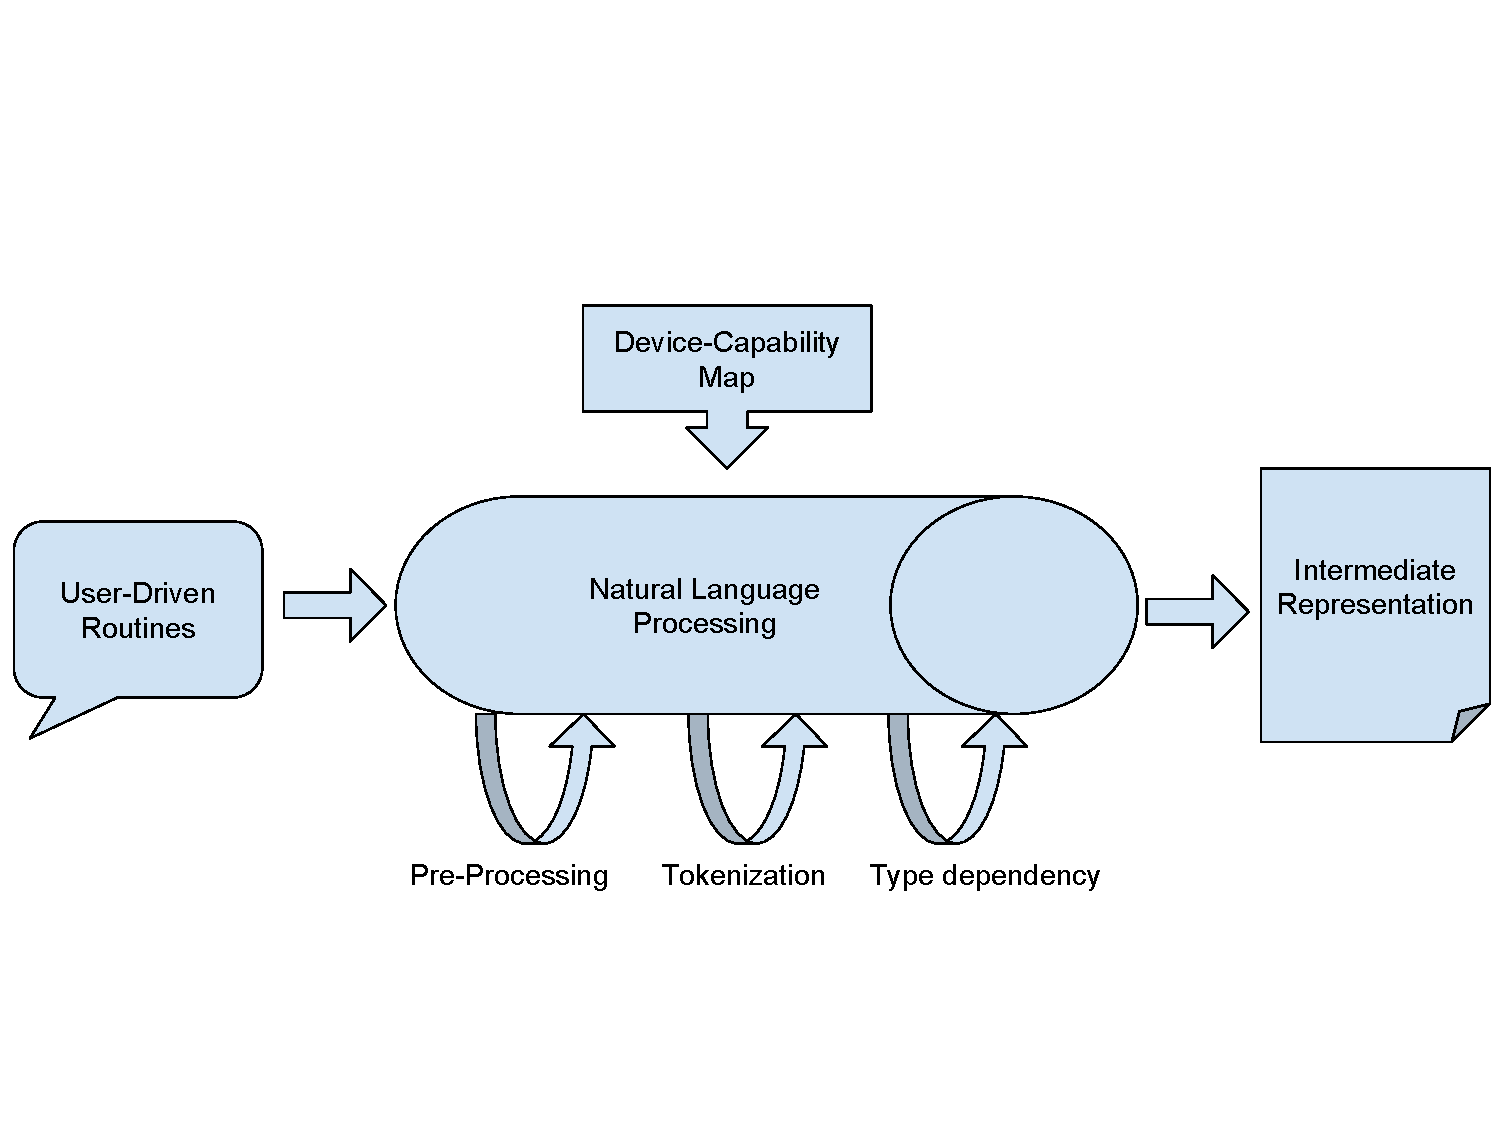
\includepdf[scale=0.5]{figs/nlp-tool.pdf}
The contributions of this paper are as follows:
\begin{itemize}
    \item We motivate the need for a holistic evaluation of home automation through the analysis of {\em user-driven routines}
    \item We develop a systematic approach that enables analysis of user-drive routines by converting them into intermediate representation. 
    \item We analyze the result of these intermediate representation and provide insights to a series of question regarding the characteristics and compositions of user-drive routines.
\end{itemize}


The remainder of this paper proceeds as follows:
In Section~\ref{sec:background}, we provide some background information on the dataset that we are using and the reason behind it.
In Section~\ref{sec:motivation}, we describe the motivation behind the transformation of user-driven routines to intermediate representation using NLP.
In Section~\ref{sec:design}, we describe the high-level design and details on each stages of our proposed approach, and our evaluation of these models follows in Section~\ref{sec:eval}. 
Section~\ref{sec:insight} provides additional insights from the generated intermediate representations.
Section~\ref{sec:discussion} discusses the limitation of the models and possible improvement for future work.
In Section~\ref{sec:related-work}, we highlight relevant related work, and 
Section~\ref{sec:conc} concludes.
